\documentclass{article}

\usepackage{Sweave}
\begin{document}
\Sconcordance{concordance:02_data.tex:02_data.Rnw:%
1 2 1 1 0 28 1}



\section{Data}

$College Scorecard$ has extensive data on colleges' admissions rates, graduation rates, and even the distribution of students based on race, income, and status from 1996 until 2015. For this project, we chose the most recent dataset, $MERGED2014_15_PP.csv$, which consists of 2014-2015 data. There are 7703 colleges in the dataset, and each college has 1743 attributes/variables of interest.

Before starting any analysis, we first cleaned the data by filtering out data we did not need. For instance, the government, our client, is only interested in analyzing graduation rates of students in public schools. As a result, we removed all private universities and colleges from our analysis. In addition, in order to use more consistent and reliable data, we futher filtered data choosing only main campuses, and colleges that award predominently bachelor degrees.

Because the data has so many variables, there are quite a few redundancies in the data. As a result, we removed quite a few variables from our dataset and only used the variables that we deemed relevant for our analysis. The predictors we selected were ACT and SAT scores, percentage of degrees awarded in each major, share of enrollment for each race, price of each college and number of students from each income group. We also created histograms for each of these quantitative variables.Below is a histogram of SAT scores for those who attended a public university:

\begin{figure}
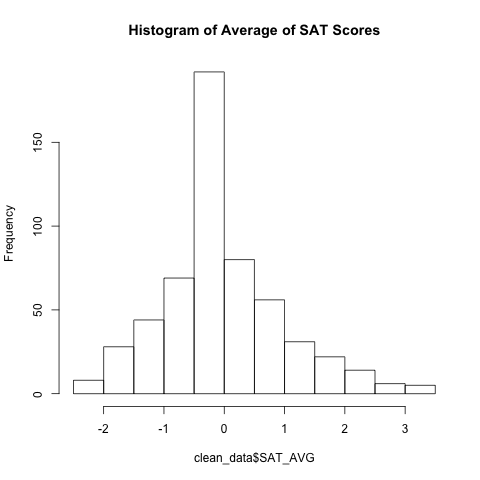
\includegraphics{../../images/histogram_SAT_avg.png}
\end{figure}

Our response variable, meanwhile, is graduation rate rate and for further analysis we included the graduation rates specific to an ethnicity (Black, Asian, Hispanic, etc.). Below, I've show histograms for the enrollment and graduation rates for each enthnicity:

\begin{figure}
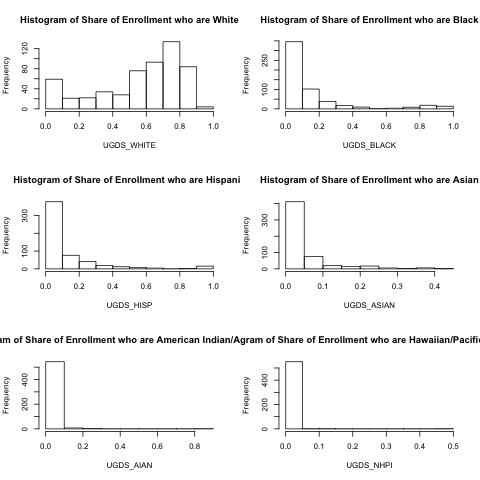
\includegraphics{../../images/histogram_race_enrollment.png}
\end{figure}

\begin{figure}
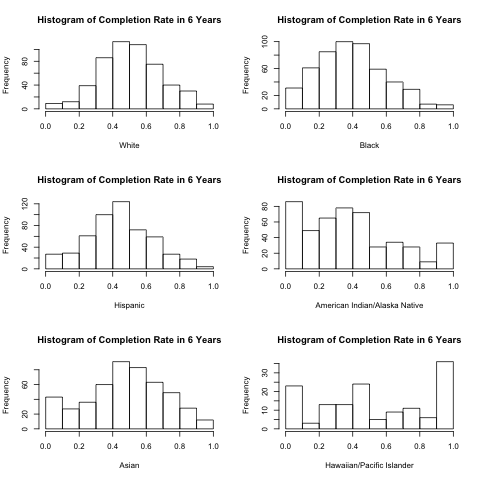
\includegraphics{../../images/histogram_race_completion.png}
\end{figure}

In the next section, I'll discuss the specific methods that we used for variable selection.

\end{document}
